\documentclass[a4paper,12pt]{scrartcl}

\usepackage[utf8]{inputenc}
\usepackage[english]{babel}
\usepackage{scrpage2}
\usepackage{amsmath,amssymb}
\usepackage{verbatim}
\usepackage{color,graphicx}
% \usepackage{hyperref}

% define common URLs
\usepackage{url}
\urlstyle{tt}
\urldef{\wwwc}{\url}{http://www.w3.org}
\urldef{\owl}{\url}{http://www.w3.org/2004/OWL/}
\urldef{\owlce}{\url}{http://www.w3.org/TR/2008/WD-owl2-syntax-20081202/#Class_Expressions}
\urldef{\carc}{\url}{http://dl-learner.org/wiki/Carcinogenesis}

\title{DL-Learner Manual [Draft]}
\author{Jens Lehmann}

\pagestyle{scrheadings}
\automark{section}

\newcommand{\todo}[1]{\textbf{[ToDo: #1]}}

\begin{document}

\maketitle

\begin{abstract}
DL-Learner is a machine learning framework for OWL and description logics. It includes several learning algorithms and is easy to extend. DL-Learner widens the scope of Inductive Logic Programming to Descriptions Logics and the Semantic Web. This manual provides the entry point to using DL-Learner and explains its basic concepts.
\end{abstract}

\tableofcontents

\clearpage

\section{What is DL-Learner?}

DL-Learner is an open source framework for (supervised) machine learning in OWL and Description Logics (from instance data). We further detail what this means:

\emph{OWL} stands for ``Web Ontology Language''. In 2004, it became the W3C\footnote{\wwwc} standard ontology language\footnote{\owl}. As such it is one of the fundamental building blocks in the Semantic Web and has been used in several scenarios on and off the web. OWL is based on \emph{description logics} (DLs), which are a family of knowledge representation languages. We refer to \cite{dlhb} for an introduction to description logics. Since OWL formally builds on description logics, we can apply DL-Learner to knowledge bases in OWL or a variety of description languages.

\emph{Machine Learning} is a subfield of Artificial Intelligence, which focuses on detecting patterns, rules, models etc.~in data. Often, this involves a training process on the input data. In \emph{Supervised} learning, this data is labelled, i.e.~we are given a number of input-output mappings. Those mappings are also called \emph{examples}. If the output is binary, then we distinguish positive and negative examples. DL-Learner as a framework is not restricted to supervised learning, but all algorithms currently build into it, are supervised.

In the most common scenario we consider, supervised learning in OWL/DLs, means that we have a background knowledge base in OWL/DLs. Additionally, we are given positive and negative examples. Each example is an individual in our knowledge base. The goal is to find an OWL \emph{class expression}\footnote{\owlce} such that all/many of the positive examples are \emph{instances} of this expression and none/few of the negative examples are instances of it. The primary purpose of learning is to find a class expression, which can classify unseen individuals (i.e.~not belonging to the examples) correctly. It is also important that the obtained class expression is easy to understand for a domain expert. We call these criteria \emph{accuracy} and \emph{readability}.

As an example, consider the problem to find out whether a chemical compound can cause cancer\footnote{see \carc{} for a more detailed description}. In this case, the background knowledge contains information about chemical compounds in general and certain compounds we are interested in. The positive examples are those compounds causing cancer, whereas the negative examples are those compounds not causing cancer. The prediction for the examples is likely to have been obtained from experiments and long-term research trials in this case. Of course, all examples have to be present in the considered background knowledge. A learning algorithm can now derive a class expression from examples and background knowledge, e.g.~this class expression in natural language could be ``chemical compounds containing a phosphorus atom''. (Of course, in practice the expression will be more complex to obtain a reasonable accuracy.) Using this class expression, we can no classify unseen chemical compounds.

\section{Getting Started}

\section{DL-Learner Architecture}

DL-Learner consists of core functionality, which provides Machine Learning algorithms for solving the learning problem, support for different knowledge base formats, an OWL library, and reasoner interfaces. There are several interfaces for accessing this functionality, a couple of tools which use the DL-Learner algorithms, and a set of convenience scripts. The general structure is illustrated in the following \ref{fig:structure}.

\begin{figure}
 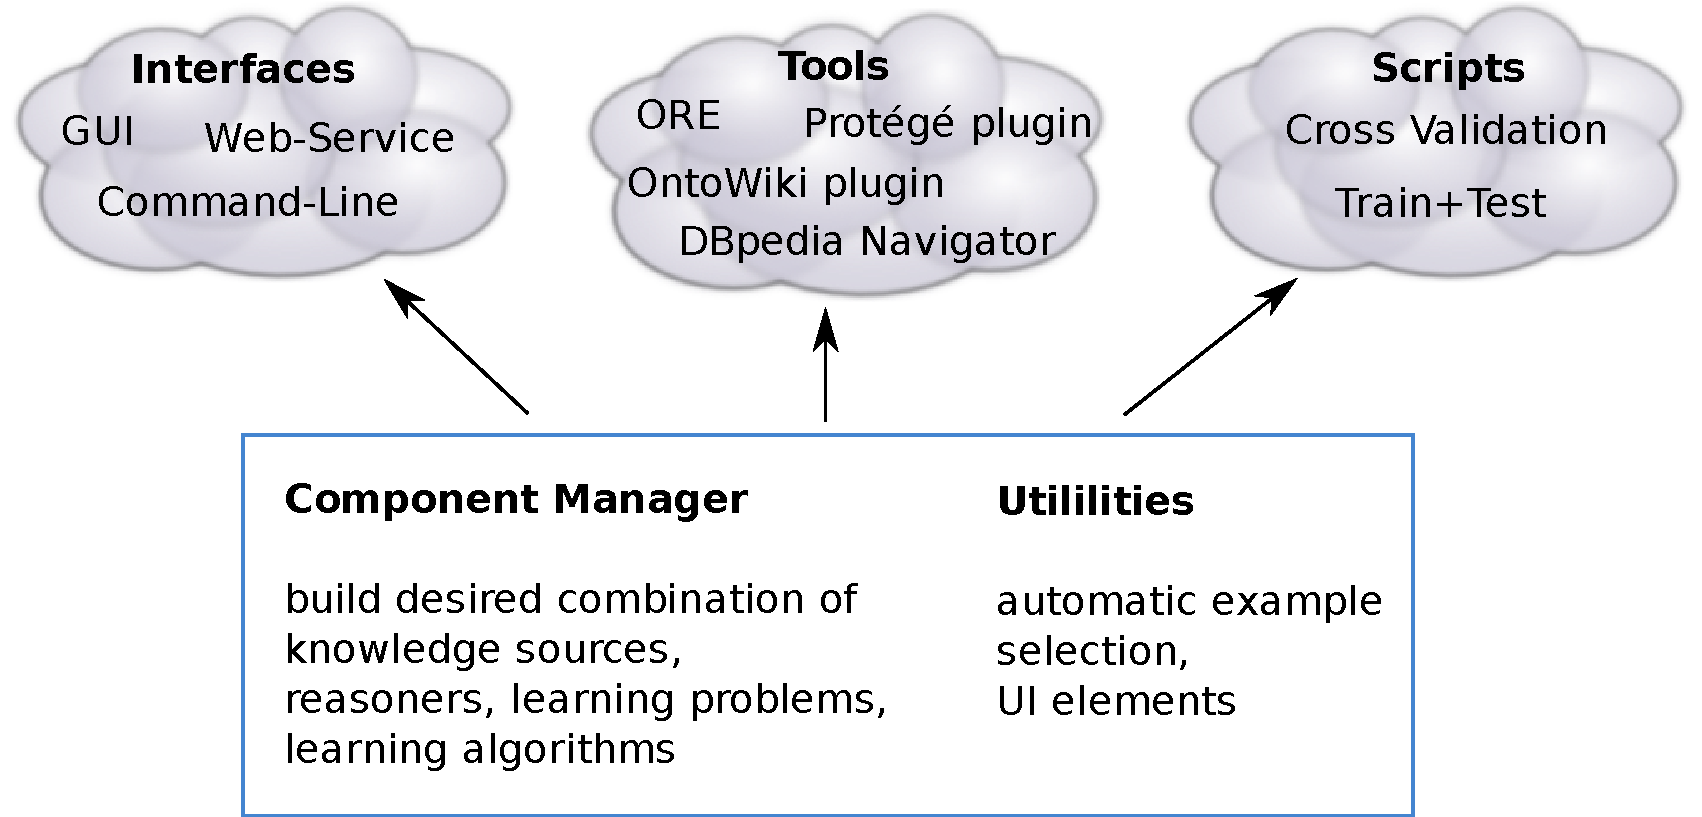
\includegraphics[width=\textwidth]{../../resources/structure_print}
 \caption{Overall structure of the DL-Learner software.}
 \label{fig:structure}
\end{figure}

To be flexible in integrating new learning algorithms, new kinds of learning problems, new knowledge bases, and new reasoner implementations, DL-Learner uses a component based model. Adding a component is as easy as subclassing the appropriate class and adding the name of the new class to the “components.ini” file (more on that in Section \ref{sec:developing}).

In DL-Learner, there are four types of components (knowledge source, reasoning service, learning problem, learning algorithm). There are several components of each type and each component can have its own configuration options as illustrated in Figure \ref{fig:components}.

\begin{figure}
 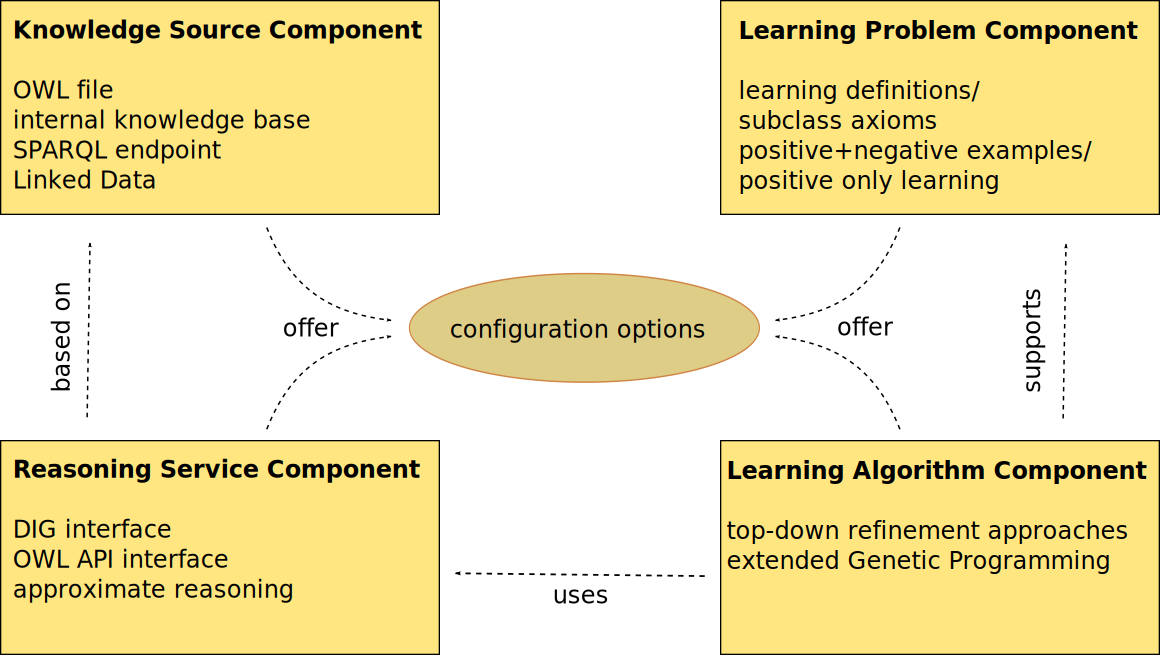
\includegraphics[width=\textwidth]{../../resources/components_print}
 \caption{The architecture of DL-Learner is based on four component types, which can each have their own configuration options. DL-Learner uses a component manager to organise all components.}
 \label{fig:components}
\end{figure}



\section{DL-Learner Components}

\subsection{Knowledge Sources}

\subsection{Reasoner Components}

\subsection{Learning Problems}

\subsection{Learning Algorithms}

\section{DL-Learner Interfaces}

\section{Extending DL-Learner}
\label{sec:developing}

\todo{example code of a simple component}

Each component can specify its own configuration options. Currently, the following configuration option types exist (new ones can be implemented if necessary):

\begin{itemize}
 \item boolean
 \item string (a set of allowed strings can be specified)
 \item int (min and max value can be specifified)
 \item double (min and max value can be specifified)
 \item set of strings
 \item list of string tuples
\end{itemize}

Although, we loose the ability to use arbitrary argument types in components, this gives us the possibility to build very flexible user interfaces. Whenever, a new component or a new configuration option for a component is added, the current user interfaces (GUI, web service, commandline) will automatically support it without any need for code changes.

\bibliographystyle{apalike}
\bibliography{bibliography}

\end{document}

